\documentclass{article}
\usepackage{graphicx}
\graphicspath{{previews/}}

\title{About ListTaskView Component}
\date{2023-12-19}
\author{ReenAG(Kim HeeSoo)}

\begin{document}
    \maketitle
    \newpage

    \begin{abstract}
        This document is for documenting how "ListTaskView" should be developed, or made.1
        It contains, if not, will be, 
        \begin{enumerate}
            \item what the Component(React) itself is for.
            \item sample image how layout of UIs.
            \item what kind of ui exists and ment to be.
            \item what props(React) it needs.
            \item what state(React) it has.
            \item etc.
        \end{enumerate}
        It's purely made for visible instructions for faster and enthusiastic development.
        In other words, it's free to manipulate whats in the document.
        But if you're first time ever doing this, be sure to add yourself in the "author" tag.\\
        Happy Coding!
    \end{abstract}

    \section{What the Component(React) itself is for}
    ListView is the main View of the GTDList.
    It will support editing and showing any existing task of the user.

    \section{Sample image how layout of UIs}
    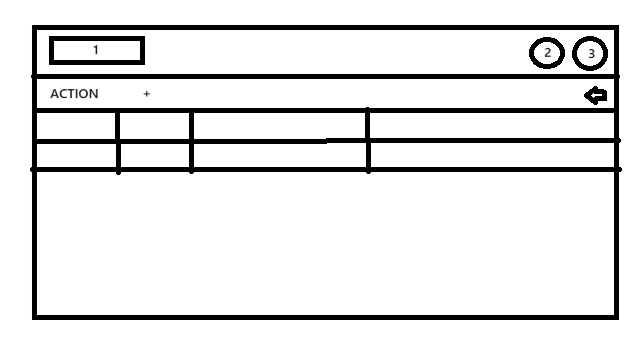
\includegraphics{listTaskView}

    \section{What kind of ui exists and ment to be}
    It includes several smaller UIs, such as :
    \begin{enumerate}
        \item title screen icon\\
        - to go back to main page(App.js)\\
        - will probably made by some kind of logo image but not specific in this point.\\
        TODO: make logo for project.
        \item menu icon\\
        - save, import/export feature.\\
        - maybe custom category making feature included.\\
        - three dot icon(with awesomefont-icon) will be used.
        \item profile icon\\
        - will lead to the profile page.
        \item task category bar\\
        - displays what tasks you have in that category and shows category name.\\
        - will have two sub-UI,(possibly Components) which is below two items.
        \item add task button\\
        - add a blank task to that included category.
        \item task\\
        - will display the "task" model like simple table, which is interactively editable.\\
        - double-click to edit a certain cell, except the below exceptions.\\
        - "check" columnm will be just click toggleable.\\
        - "difficulty" columnm displays the float number by integer, with "+" sign to give a hint about the floating number.
    \end{enumerate}

    The preview of the view could be shown in here.


\end{document}